\Chapter{A játék fejlesztésének menete}

A Monopoly játék stratégiáinak vizsgálatához először magát a játékot kellett leprogramozni. Ezt \textit{Vue} keretrendszer segítségével készítettem el \textit{JavaScript} programozási nyelven. A fejezetben ennek a megtervezéséről olvashatunk.

\Section{Fejlesztés előkészítése}

Miután kialakult egy konkrét elképzelés a szakdolgozat témájával kapcsolatosan, összegyűjtöttem a legfontosabb szempontokat, hogy mikre kell a legnagyobb figyelmet fordítanom a program implementálása során. Alaposan átolvastam a Monopoly játék eredeti szabályait \cite{coombs1987markup}, és az általam elgondolt online megvalósítás lehetőségeivel összefésültem. Célom ezzel az volt, hogy a játék online verzióban is izgalmas, kiegyensúlyozott élményt nyújtson. Készítettem egy tervet a játék megvalósításának lépéseiről, ami nagyban segített abban, hogy hol lesznek esetleges nehézségek a fejlesztés során.

Ennek a folyamatábrának a megalkotásával próbáltam megtervezni, hogy hogyan fog kinézni maga a játék menete programozási szempontból. \Aref{fig:flowchart}. ábrán láthatunk egy folyamatábrát, amely lényegretörően összegzi a játékmenetet. (Elkészítéséhez a \textit{draw.io} nevezetű folyamatábra készítő ingyenes internetes programot használtam, mely nagyban megkönnyítette a feladatomat a fejlesztés további szakaszaiban.)

A backend illetve a frontend részek megírása párhuzamosan ment, mivel így lehetőség adódott teljes értékű funkciókat kipróbálni már az előtt, hogy a teljes frontend vagy backend elkészült volna. Ebből kifolyólag a tesztelési fázisok is azonnal megtörténtek, így az előforduló hibákat kisebb kód részben kellett keresnem és javítanom. Abban az esetben, ha a programnak több komponensét szerettem volna összekapcsolni előfordult, hogy néhány függvényt vagy osztályt egy az egyben újra kellett gondolnom. Ezeket a lépéseket folyamatosan dokumentáltam, ami segített abban, hogy utólag visszaolvasva is lássam, hogy mit miért kellett javítanom.

\begin{figure}[h!]
\centering
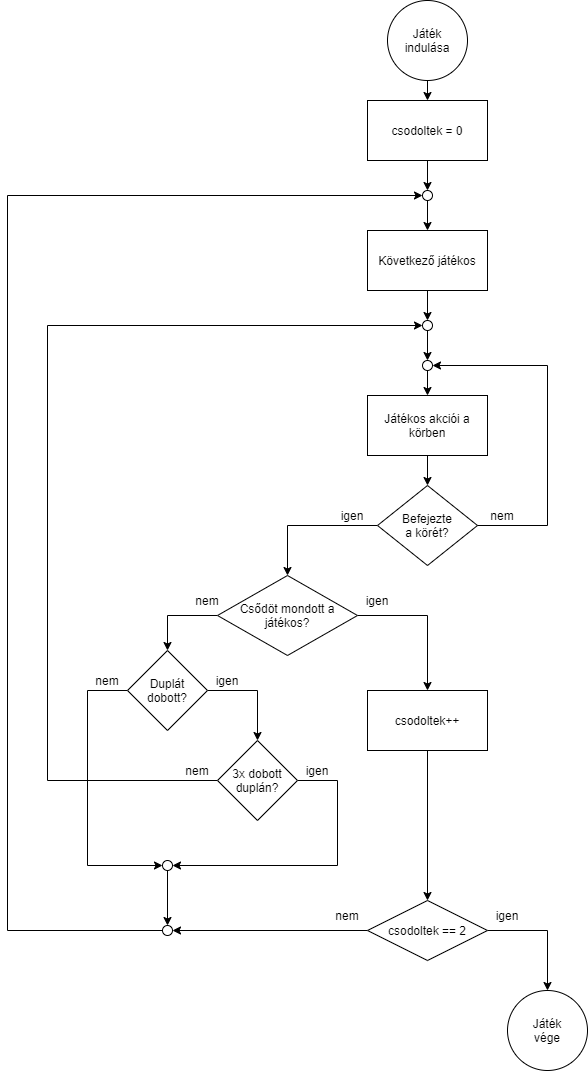
\includegraphics[scale=0.6]{images/folyamata.png}
\caption{A játék folyamatábrája}
\label{fig:flowchart}
\end{figure}

\newpage
\Section{Fejlesztés menete}

Az első lépések közé tartozott a NodeJS szoftverrendszer telepítése, illetve a \textit{VueJS} JavaScript keretrendszer \texttt{npm}-el történő installálása \cite{cantelon2014node}.

Ez után létrehoztam egy teljesen alap, sablon \textit{Vue} projektet, ami a későbbiekben magának a frontend résznek az alapját képezi. Ezzel együtt egy \texttt{server.js} fájlt is elkészítettem, mely magát a szervert alkotja. Az \textit{Express} keretrendszer segítségével készült \cite{teixeira2012professional}. Miután ezek a lépések megtörténtek, beépítettem a \textit{socket.io} nevezetű valós idejű kliens-szerver kommunikációt segítő javascript keretrendszert. Erre azért volt szükség, mert a tervezési fázisban már tudtam, hogy szükségem lesz arra, hogy a szerver több klienst is ki tudjon szolgálni egyszerre valós időben.

Felhasználói szempontból az első feladat egy bejelentkező felület elkészítése volt. Ennek megvalósításához egy \texttt{Login.vue} komponenst hoztam létre és importáltam az \texttt{App.vue} alkalmazásba. A \texttt{Login.vue}-n keresztül kapott adatokat át kellett adni az \texttt{App.vue}-nak, hogy az továbbítani tudja a szerver felé ezeket, hiszen maga a komponens nem áll kapcsolatban közvetlen a szerverrel. Az elsőként bejelentkezett játékos a HOST titulust viseli, ő indítja a játékot, illetve képes parancsok használatára.

Szükség volt egy Chat felület megvalósítására ahol a játékosok információkat látnak a játékkal kapcsolatban, illetve kommunikálni is tudnak egymással. Ezt a felületet használtam arra is, hogy jobban megismerkedjek a \textit{socket.io} lehetőségeivel, és tesztelni tudjam annak működését. Ezen a felületen van lehetősége a HOST-nak parancsok kiadására (pl.: ‘/start’ - A játék indítása).

A játék kezdete előtt a játékosok egy úgynevezett várakozó szobába kerülnek, ezért a következő teendő ennek az elkészítése volt. Lényegében erre azért volt szükség, hogy összegyűljön a négy játékos a játék kezdetéhez.

A grafikus felület elkészítése is fontos része volt a folyamatnak. Egy átlátható, könnyen kezelhető alkalmazás létrehozása volt a célom. Törekedtem az egyedi megvalósításokra, a webes megjelenítésekhez \textit{Bootstrap} keretrendszert, illetve egyéni CSS-t alkalmaztam. A képi elemek megvalósításához az \textit{Adobe Photoshop 2020} nevezetű programot használtam, már itt fontosnak tartottam azt, hogy mindenből meglegyen a \texttt{.psd} fájl is, ha esetlegesen szerkesztenem kellene.

A szerveren belül megvalósítottam, hogy tárolja a bejelentkezett játékosokat, és folyamatosan frissítse azok állapotát minden kliens felületén. A program ezen állapotában még csak egy \texttt{players} nevű tömb tárolta a játékosok paramétereit, és a játék állását pedig változók a \texttt{server.js}-n belül.

Elkészítettem a \texttt{Table.vue} komponenst, ami megjeleníti a játék aktuális állását, a táblát és a rajta elhelyezkedő bábúk helyzetét. Emellett ebben a komponensben helyeztem el a játékos által használható gombokat (pl.: “Dobás” - Dobás a kockával). Ebben a fejlesztési szakaszban került sor arra is, hogy paraméterezzem a bábúk helyzetét az aktuális mezőre lépéskor, ez viszonylag aprólékos feladat volt. A szerverben megvalósításra került a következő aktív játékos beállítása, illetve frissítése a kliensek számára is. A szabályzathoz igazítva a dupla illetve tripla dobások lehetőségét is figyelembe véve. Itt több tesztelésre is sor került, ez a fázis tekinthető a játék első prototipusának. Ekkorra éreztem azt, hogy kellően megismertem a használt keretrendszerek lehetőségeit.

A program elérkezett abba a fázisba, hogy objektum orientált legyen. Létrehoztam külön osztályokat a \texttt{classes} mappába. Ezek voltak a \texttt{Game}, \texttt{Player}, \texttt{PlayerManager}, \texttt{Property}, \texttt{Table} nevezetű osztályok. A szerveren belül illetve az \texttt{App.vue}-ban is ezeknek megfelelően lettek átgondolva az eddig megvalósított funkciók, és sokkal átláthatóbb lett a kódolás.

Egy nagyobb fejlesztés következett, a bizniszek kidolgozása. Minden ezzel kapcsolatos dolog megvalósításra került (vásárlás, fizetés, eladás). Ennek mintájaként a telkek, illetve szolgáltatók is hasonlóképpen készültek el, hiszen a logikai felépítésük nem tért el sokban.

A kereskedés funkció volt az utolsó dolog ami nagyobb kihívást jelentett számomra, hiszen itt két játékos közötti kommunikációt kellett megvalósítani a szerveren keresztül. Ennek a megvalósítása viszonylag időigényes volt, de mire idáig eljutottam a fejlesztésben már kellő tapasztalatra tettem szert az alkalmazást illetően.

Innen már csak apróságok választottak el az 1.0-s verziótól, ezek pedig inkább a kreatív részét képezték a fejlesztésnek. Kitaláltam a mezőneveket, illetve hogy mik szerepeljenek a szerencsekártyákon, elkészítettem ezek implementációját.

Utolsó simításként a játék vége, a csőd megalkotása maradt hátra, ami egy nagyon egyszerű folyamatként sikerült, és mivel elsőre sikerült úgy megírni ahogy elterveztem, jöhetett is magánk a játéknak a tesztelése, egyelőre még csak botok nélkül.

A tesztelés úgy zajlott, hogy négyen játszottunk külön eszközökről, ugyanarról a hálózatról. Körülbelül maga a tesztelés 4-5 órát vett igénybe, nagyjából 10-14 játékot játszottunk, viszont valamelyik csak pár percig tartott a talált problémák miatt. Azokat a hibákat, amik befolyásolták a játék menetét rögtön javítottam.

Ilyen volt például, hogy az alkalmazás rosszul kezelte a kör átadását tripla dobás esetén. Viszont ami csak úgymond formailag tett hozzá a játékhoz, azokat kigyűjtöttük egy lapra, hogy a tesztelés után sorban tudjam javítani a felírt dolgokat, emellett az is felkerült a papírra, hogy hol és mikor jelentkeztek az adott hibák. Amikor a talált hibák kijavításra kerültek, elkezdődött a botok megírása.

Kezdetben egy olyan botra volt szükségem, ami képes alap funkciók végrehajtására. Ez alatt a dobást, kör átadását, illetve a börtönből való szabadulást, csődöt értem. Külön osztályt kapott \texttt{BotEasy} néven, és tudtam, hogy a továbbiakban ezt fogom továbbfejleszteni. Három különböző nehézségű bot megvalósítását terveztem, így el kellett döntenem, milyen funkciókban fognak főként eltérni egymástól.

Soron következő megvalósítású botom a \texttt{BotMedium} osztályt kapta. Már képes volt a táblán lévő összes megvásárolható biznisz/szolgáltatás/telek megvételére, és válogatás nélkül élt is a lehetőséggel. Lehetőséget adtam neki, hogy fejleszteni illetve bontani tudja a telkeket, esetenként eladni azokat, hogyha csőd közeli helyzetbe kerül.

Végezetül, a legerősebb bot a \texttt{BotHard} osztályt tudhatja magáénak. Nagyban hasonlít a \texttt{BotMedium} osztályra, viszont ők már paraméterezve vannak. Kialakításuk során gondolnom kellett arra, hogy a leendő szimulációkban ők foglalnak majd helyet.

\newpage
\Section{A projekt felépítése}

A projekt szerkezete a \textit{Vue} hivatalos ajánlása szerint épül fel, így annak részleteire nem tünt szükségesnek kitérni, azt a \textit{Vue} keretrendszer hivatalos dokumentációja tartalmazza \cite{filipova2016learning}.

\Aref{fig:project_structure}. ábrán láthatjuk a \textit{Vue} és az Express projekt struktúráját, benne a komponenseket és a \textit{JavaScript} osztályok definícióit tartalmazó modulokat.

\begin{figure}[h!]
	\centering
	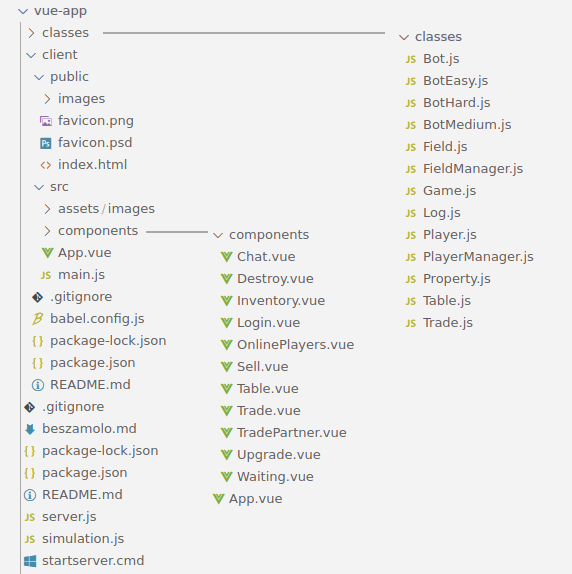
\includegraphics[scale=3]{images/project_structure.png}
	\caption{Az elkészített projekt struktúrája fájlrendszer szintjén}
	\label{fig:project_structure}
\end{figure}

A következő fejezetekben ennek a részletezésére, a felépítés és működés részletes áttekintésére kerül majd sor.
